\chapter{Vector Functions} \label{chap:vector}

\section{Element-wise operators}

Often, we are tasked we computing the gradient of a function $\phi: \real^n \to \real^n$ that takes the form of an \textit{element-wise operator}.  By this, we mean that there exists some scalar function $f:\real \to \real$ such that for any $\xx \in \real^n$

\begin{align}
  [\phi(\xx)]_i = f(\xx_i), \quad \forall i \in \{1, \dots, n\}
\end{align}

For these operators, it is helpful to first compute the derivative of the scalar component function,~$f'$.  This can then be used in combination with differentials to compute the gradient of $\phi$ as follows:

\begin{align}
  \underbrace{{\dd}\phi(\xx)}_{n \times 1} = \underbrace{\diag(f'[\xx])}_{n \times n} \underbrace{\vphantom{(}{\dd
}\xx}_{n \times 1} \label{eqn:eltwise-differentials}
\end{align}

where we have used the notation $f'[\xx]$ to denote that $f'$ is applied element-wise to each element of $\xx$ (this notation is used throughout the document), and the dimensions of each term are displayed beneath the equation. 


\section{Sigmoid}

The sigmoid function is often used as an elementwise operator in neural networks.  The sigmoid is a scalar map $\sigma : \real \to \real$ defined by: 

\begin{align}
\sigma (x) = \frac{1}{1 + e^{-x}} = \frac{e^x}{1 + e^x}  
\end{align}


We can compute its gradients using the quotient rule:

\begin{align*}
  \dd (\sigma(x)) &= {\dd} \bigg(\frac{e^x}{1 + e^x}\bigg) \\
                  &= \frac{(1 + e^x) \dd (e^x) - e^x \dd (1 + e^x)}{(1 + e^x)^2}
               = \frac{(1 + e^x)e^x \dd x - e^x e^x \dd x}{(1 + e^x)^2} \\
               &= \Bigg(\frac{e^x((1 + e^x) - e^x)}{(1 + e^x)^2}\Bigg)\dd x = \Bigg(\frac{e^x}{(1 + e^x)}\frac{1}{(1 + e^x)}\Bigg){\dd} x \\
               &= \sigma(x)(1 - \sigma(x)) {\dd} x \\                              
\end{align*}

which tells us that $\sigma'(x) = \sigma(x) (1 - \sigma(x))$.  The sigmoid and its derivative are shown in Fig.\ref{fig:sigmoid}.  We can now apply Eqn.\ref{eqn:eltwise-differentials} to obtain the Jacobian of the element-wise sigmoid:

\begin{align}
\dd (\sigma[\xx]) = \diag\Big(\sigma[\xx]\circ(\bone - \sigma[\xx])\Big){\dd} \xx
\end{align}

Since the diagonal matrix is symmetric, it follows that $\nabla \sigma(\xx) = \diag\Big(\sigma[\xx]\circ(\bone - \sigma[\xx])\Big)$.

\begin{figure}
\centering
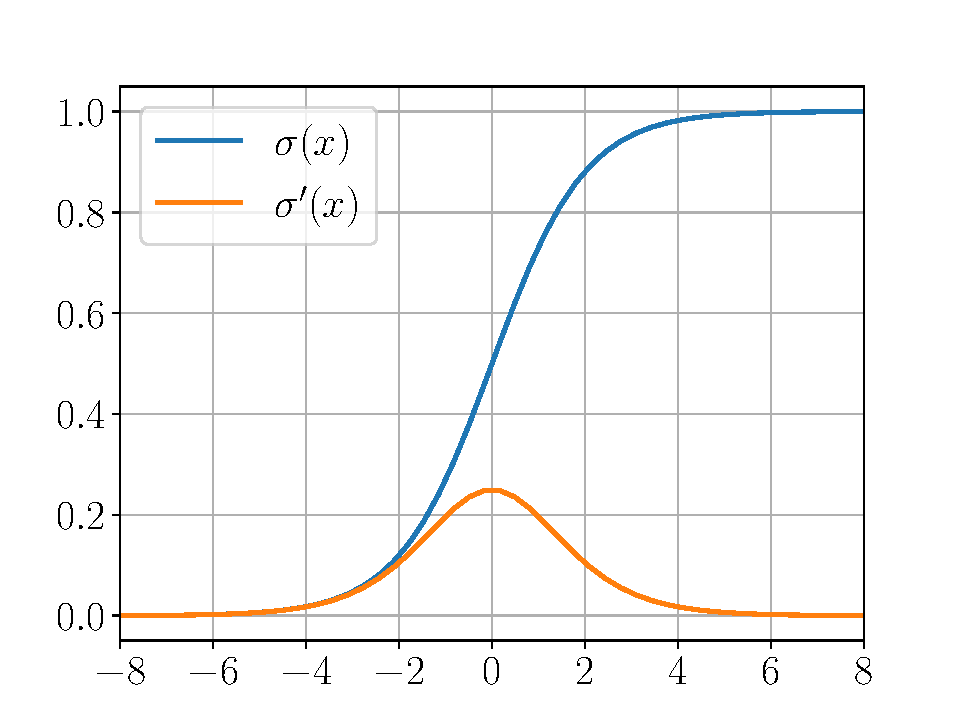
\includegraphics[width=0.5\textwidth]{figs/sigmoid.pdf}
\caption{The sigmoid function and its derivative.\label{fig:sigmoid}}  
\end{figure}

\section{Softmax} \label{sec:softmax}

The softmax function represents another vector function that is commonly used as a computational block in neural networks.  It can be viewed as a form of generalised sigmoid (for this reason it is common to overload the $\sigma$ symbol for the softmax, $\sigma : \real^n \to \real^n$).  It may be helpful to keep in mind that although it produces an output with the same shape as its input, it is not an element-wise operator and $\sigma(\xx) \neq \sigma[\xx]$ (i.e. it does not produce the same output as an element-wise sigmoid).  It is defined by:

\begin{align}
\sigma (\xx) = \frac{\exp[\xx]}{\bone^T \exp[\xx]} 
\end{align}

Note that the denominator here is a scalar, while the numerator has shape $n \times 1$.  To compute the gradient of this function, we can proceed with differentials:

\begin{align}
  \dd(\sigma(\xx)) &= \dd \Bigg( \frac{\exp[\xx]}{\bone^T \exp[\xx]} \Bigg) \\
                 &= \frac{(\bone^T \exp[\xx]) \dd (\exp[\xx]) - \exp[\xx] \dd (\bone^T \exp[\xx])}{(\bone^T \exp[\xx])(\bone^T \exp[\xx])} \\
                 &= \frac{(\bone^T \exp[\xx]) \diag(\exp[\xx]){\dd} \xx - \exp[\xx] (\bone^T \diag(\exp[\xx]){\dd}\xx)}{(\bone^T \exp[\xx])(\bone^T \exp[\xx])} && \text{(using \ref{eqn:eltwise-differentials})}\\
                 &= \Bigg(\frac{\diag(\exp[\xx])}{(\bone^T \exp[\xx])} - \frac{\exp[\xx] (\bone^T \diag(\exp[\xx]))}{(\bone^T \exp[\xx])(\bone^T \exp[\xx])}\Bigg){\dd}\xx \\
                  &= \Bigg(\diag(\sigma(\xx)) - \sigma(\xx)\sigma(\xx)^T\Bigg){\dd}\xx && \text{(using \ref{eqn:diagLinear})} \label{eqn:vectorSoftmax}
\end{align}

Since both terms are symmetric matrices, it follows that $\nabla\sigma(\xx) = \diag(\sigma(\xx)) - \sigma(\xx)\sigma(\xx)^T$.  

There are also often cases where we would like to apply the softmax operator to a higher order tensor.  The simplest way to address this notationally is define the softmax operator $\sigma(\cdot)$ to always act along the first non-singleton dimension. Thus for an $m \times n$ matrix $X = [\xx_1 | \dots | \xx_n]$ (with each $\xx_i \in \real^m$), the action of the softmax operator produces the following effect:

\begin{align*}
  \sigma(X) &= \sigma \Big( \left[\begin{array}{c|c|c}
  \xx_1 & \dots & \xx_n
\end{array}\right] \Big) \\
 &= \left[\begin{array}{c|c|c}
  \sigma(\xx_1) & \dots & \sigma(\xx_n)
\end{array}\right]
\end{align*}

We can derive the gradient of this operator with respect to an input matrix $X \in \real^{m \times n}$, using the vec operator. This is a little more involved than the previous derivations, so the equations are interspersed with visualisations.  The overall strategy is to reach an expression of the form $\dd \vv(\sigma(X)) = A \dd \vv(X)$ and apply the identification theorem \citep{magnus1988matrix} to read off the Jacobian of the softmax as $A \in \real^{mn \times mn}$.

\begin{align}
  \dd(\vv(\sigma(X))) &= \dd \big( \left[\begin{array}{c}
  \sigma(\xx_1) \\
  \vdots \\
  \sigma(\xx_n)
\end{array}\right] \big) =
\left[\begin{array}{c|c|c}
  \dd (\sigma(\xx_1); \xx_1) & \hdots & {\dd} \sigma(\xx_1; \xx_n) \\
  \hline
  \vdots & \ddots & \vdots \\
  \hline  
  \dd (\sigma(\xx_n); \xx_1) & \hdots & \dd(\sigma(\xx_n); \xx_n) \\
\end{array}\right] \label{eqn:matrixSoftmax}
\end{align}

Here, we are writing the differential operator $\dd(\cdot ; \cdot)$ with an explicit dependence on its increment as the second argument (i.e. as defined in Eqn.~\ref{eqn:vecDifferential}), rather than leaving this to be determined implicitly as was done previously.  The off-diagonal terms disappear so we are left with the block diagonal matrix $A$ where block $ii$ contains $\dd(\sigma(\xx_i); \xx_i)$ i.e. the vector differential of the softmax. 

We therefore see that the $\sigma(\cdot)$ operator has several different meanings depending on the shape of its input (e.g. sigmoid, standard vector softmax, column-wise softmax for scalars, vectors and matrices respectively). Thus we can replace the last term in Eqn.~\ref{eqn:matrixSoftmax} with the differentials found in Eqn.~\ref{eqn:vectorSoftmax} to proceed:

\begin{align}
= \left[\begin{array}{c|c|c}
  \diag(\sigma(\xx_1)) - \sigma(\xx_1)\sigma(\xx_1)^T \dd \xx_1 & \hdots & 0_m \\
  \hline
  \vdots & \ddots & \vdots \\
  \hline  
  0_m & \hdots & \diag(\sigma(\xx_n)) - \sigma(\xx_n)\sigma(\xx_n)^T \dd \xx_n \\
\end{array}\right]  
\end{align}

where $0_m$ denotes an $m \times m$ matrix of zeros. We can summarise this a little more concisely as follows:

\begin{align}
  \dd(\vv(\sigma(X))) = \Bigg(\diag(\sigma(X)) - (I_n \otimes \underbrace{\bone \bone^T}_{m \times m}) \circ (\sigma(X)\sigma(X)^T)\Bigg) {\dd}\vv(X) \label{eqn:matrixSoftmaxDiff}
\end{align}

We see that the resulting Jacobian closely mirrors that of the vector function derived in Eqn.~\ref{eqn:vectorSoftmax}, except that there is an additional block matrix of ones that prevents enforces that partial derivatives are zero between elements in the outputs of one column and elements in the inputs from different columns.
